\section{Le future du Big Data}
Ses dernières années, plusieurs articles parlent de la fin du Big Data à cause de certains singes, comme le fait qu’Apache est décidé d’abandonné une dizaine de projets Hadoop.

Pris individuellement, le fait de retirer un projet peut sembler négligeable. Cependant, il est ici question de 13 logiciels, ce qui est un événement assez significatif. Voici, par ordre alphabétique, la liste des projets Apache Hadoop ayant fait l’objet d’un retrait : \textbf{Apex, Chukwa, Crunch, Eagle, Falcon, Hama, Lens, Marmotta, Metron, PredictionIO, Sentry, Tajo et Twill}. Alors que ces programmes sont liés au big data, la société a annoncé le 1er avril le retrait d’au moins 19 projets open source de sa réserve. Parmi ces derniers, une dizaine figure dans l’écosystème Hadoop.

Gartner considère quant à lui que les entreprises qui reposent sur de larges quantités de données historiques ont réalisé avec la pandémie que la plupart de leurs modèles ne sont plus pertinents. « La pandémie a tout changé, rendant beaucoup de données inutiles » expliquent les analystes.

Dépassées sont les techniques traditionnelles d’IA reposant sur des données historiques massives ! L’avenir est à des technologies d’analyse et d’IA qui requièrent moins de données, mais davantage de diversité. Il est temps de passer du « Big Data » au \textbf{« Small \& Wide Data »}.

C’est l’une des grandes tendances mises en lumière par le nouveau rapport Gartner sur les 10 tendances \textit{ « Data \& Analystics »} pour 2021. \textit{ « Ces tendances peuvent aider les organisations et la société à faire face aux changements perturbateurs, à l’incertitude et aux possibilités qu’elles offrent pour les trois années à venir »} explique Rita Sallam, VP Analyst chez Gartner.

\begin{figure}[h]
	\centering
	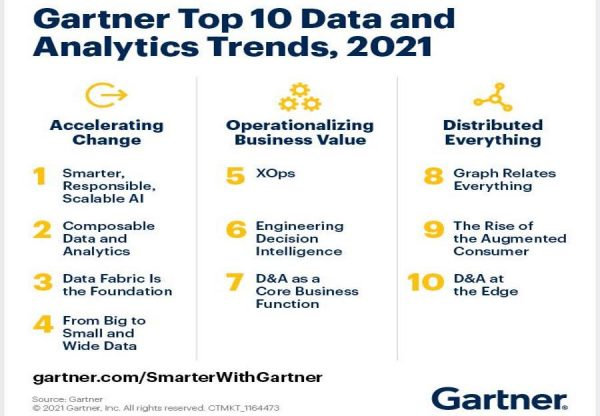
\includegraphics[scale=0.6]{img/part1/1.12}
	\caption{les 10 tendances « Data \& Analystics »}
\end{figure}